\documentclass[a4paper,10pt]{scrartcl}

\usepackage[utf8]{inputenc}
\usepackage[ngerman]{babel}
\usepackage[T1]{fontenc}
\usepackage{amsmath}
\usepackage[section]{placeins}
\usepackage{graphicx}
\usepackage{esvect}
\usepackage{amssymb}



\title{Praktikum B Vorbereitung zu Versuch "fp"}
\author{Leon Machtl und Raphael Lehner}
\date{21.11.2019}

\begin{document}
	\maketitle
	\tableofcontents
	\newpage
	
	\section{Einleitung zum Versuch}
	In diesem Versuch werden Interferenzphänomene mit Hilfe eines Fabry-Perot-Interferometers betrachtet. Unter anderem wird die Wellenlänge eines Lasers bestimmt. Ein solches Interferometer besteht normalerweise aus zwei parallelen Spiegeln, die teildurchlässig sind. Diese spiegelnden Flächen stellen einen optischen Resonator dar. In diesem Versuch wird ein Laserstrahl mit einer Linse aufgeweitet und anschließend durch eine Streuscheibe in verschiedenen Winkeln gestreut. Das so gestreute Licht trifft dann in einem Winkel auf die erste teildurchlässige Fläche. Der transmittierte Anteil eines Lichtstrahls wird dann zwischen den beiden Spiegeln mehrmals reflektiert, wobei bei jeder Reflexion ein gewisser Anteil transmittiert. Der reflektierte Anteil legt dabei einen längeren Weg zurück. Die transmittierten Anteile des Strahls werden anschließend mit einer Linse auf einen Schirm gebündelt, wo sie entweder konstruktiv oder destruktiv miteinander interferieren. Diese Interferenz wird durch den Einfallswinkel des Lichts und dem Verhältnis des Plattenabstands zur Wellenlänge bestimmt, somit ergibt sich für das gestreute Licht ein ringförmiges Interferenzmuster auf dem Schirm. \\
	Lässt man den Plattenabstand auf einem bekannten konstanten Wert, so kann man das Fabry-Perot-Interferometer als Kalbriernormal (Etalon) für spektroskopische Geräte benutzen, da unter einem gegebenem Ausfallswinkel nur eine Wellenlänge passieren kann, welche direkt proportional zum Spiegelabstand ist, da sich andere Wellenlängen durch die Interferenz abschwächen oder aufheben.\\
	Wenn beide Spiegel beweglich sind, spricht man eigentlich von einem Interferometer. Im Fall eines konstanten einfallenden Spektrums kann man durch das Verstellen des Spiegelabstandes beliebige Wellenlängen aus dem Spektrum herausfiltern, sowie durch Messung des Spiegelabstandes die Wellenlänge bestimmen. Das Fabry-Perot-Interferometer funktioniert dann als Schmalbandfilter.
	\begin{figure}[h]
\centering
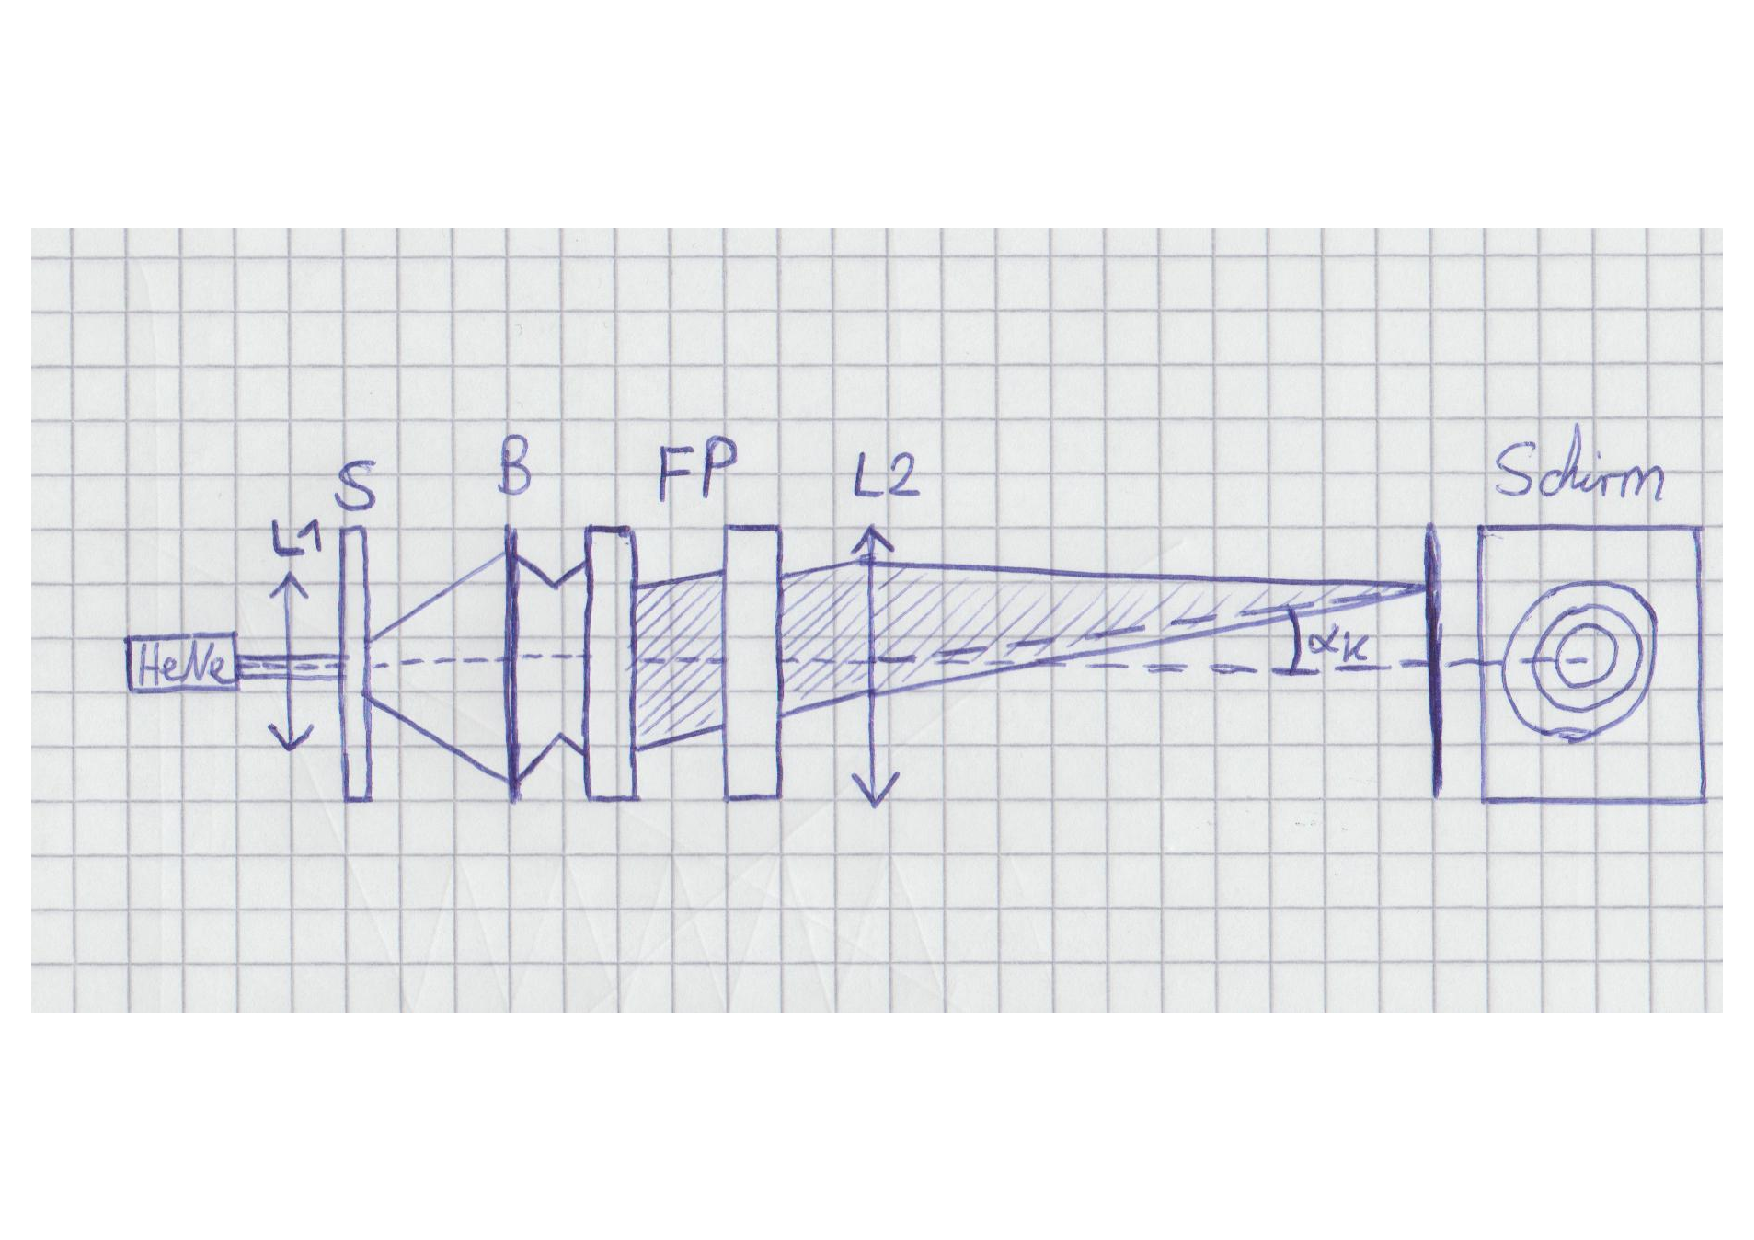
\includegraphics[width=0.9\textwidth]{./Bilder/fp1}
\caption{Fabry-Perot-Interferometer}
\end{figure}
\FloatBarrier
	
	\subsection{Interferenzen gleicher Neigung}
	Man spricht von Interferenzen gleicher Neigung, wenn ein Lichtbündel mit unterschiedlichen Strahlrichtungen
	auf zwei parallele Grenzflächen fällt. Bei dieser Art der Interferenz resultieren die Interferenzmuster aus der Variation
	des Gangunterschieds zwischen den interferierenden Teilwellen mit dem Einfallswinkel der Strahlung. Die Situation ist in folgender Skizze dargestellt.\\
	\\
	Der Gangunterschied beträgt somit
	\begin{align*}
	\Delta s=2dcos(\alpha)
	\end{align*}
	Somit folgt für die Phasendifferenz
	\begin{align*}
	\delta=\frac{2\pi \Delta s}{\lambda}=4\pi d cos(\alpha)\frac{1}{\lambda}
	\end{align*}
	Es ergeben sich also konstruktive Interferenzen, wenn der Gangunterschied ein geradzahliges Vielfaches von \(\frac{\lambda}{2}\) ist und destruktive Interferenzen für ungeradzahlige Vielfache.
	\begin{figure}[h]
\centering
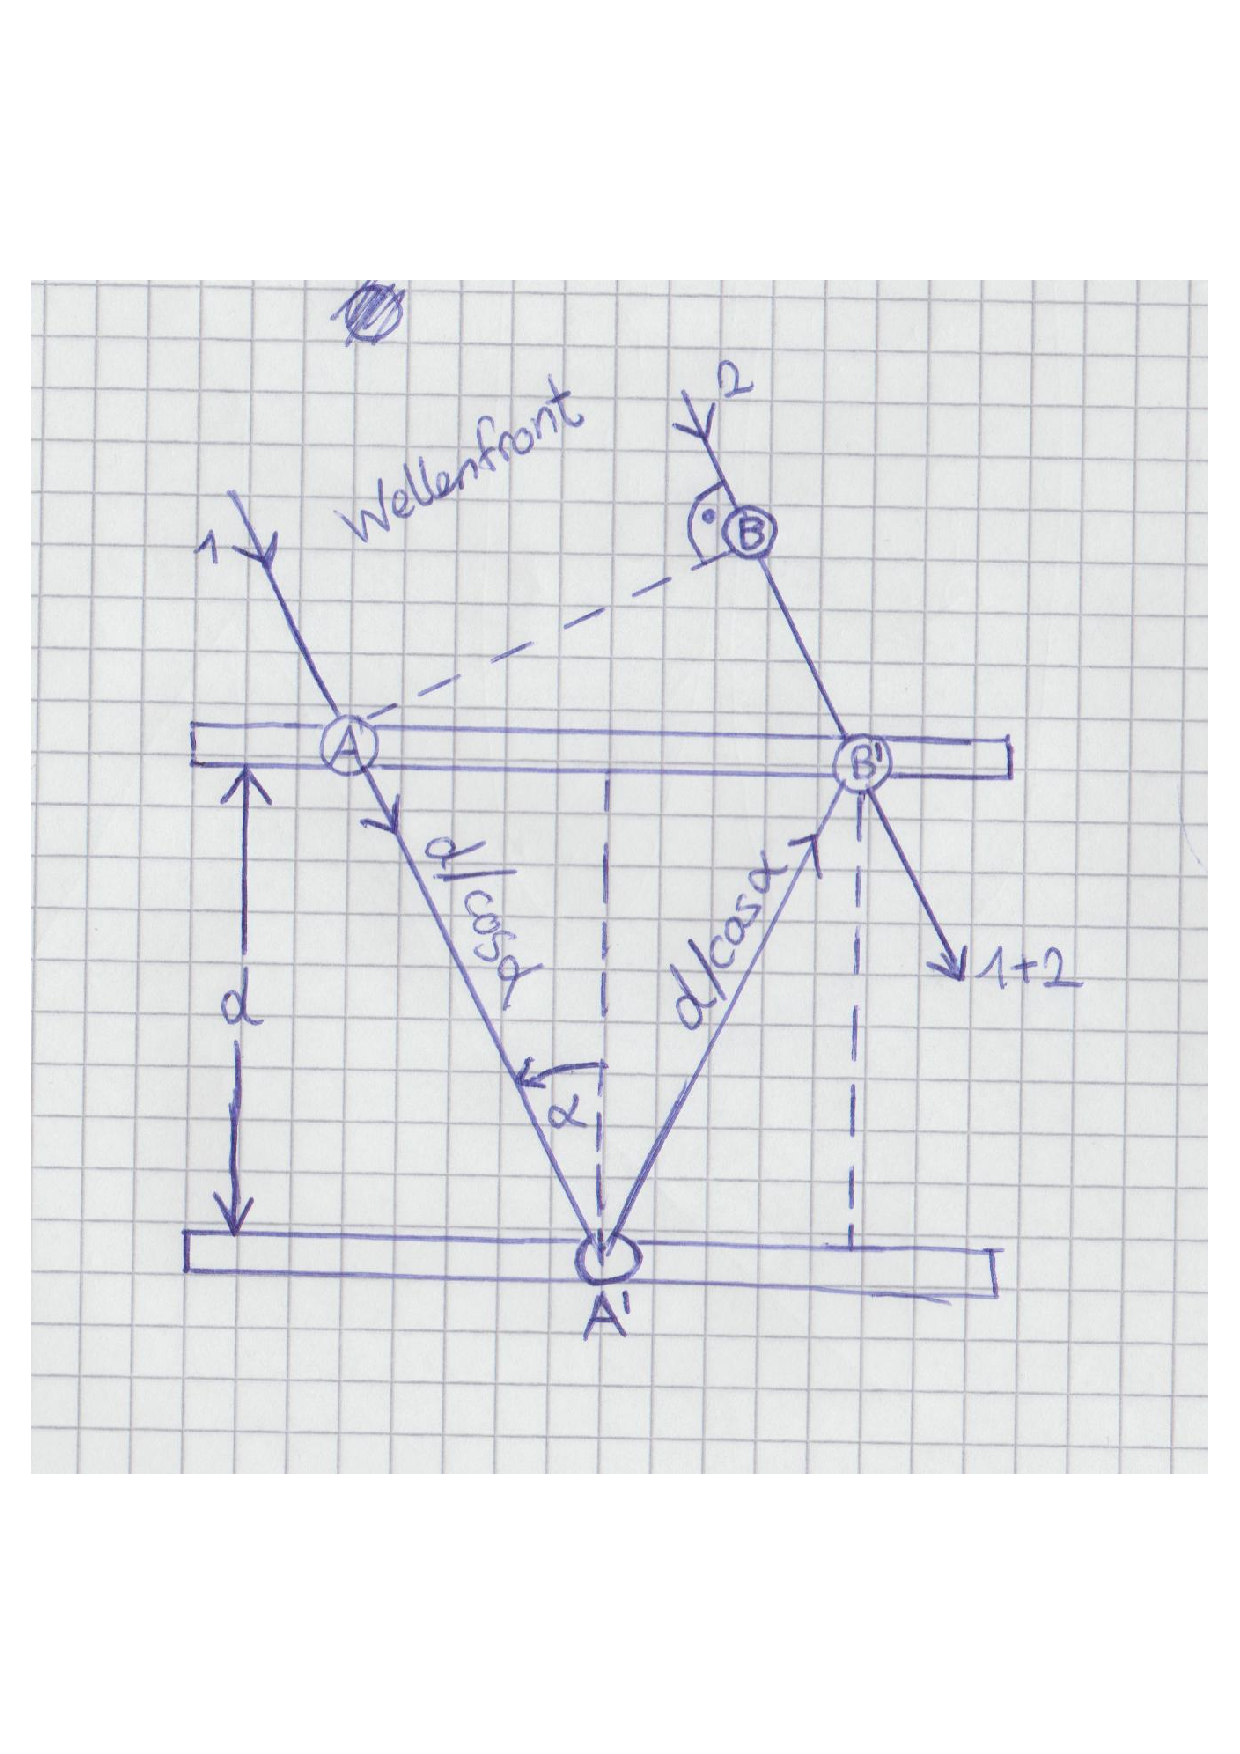
\includegraphics[width=0.9\textwidth]{./Bilder/fp2}
\caption{Interferenzen gleicher Neigung}
\end{figure}
\FloatBarrier
	
	\subsection{Vielstrahlinterferenz}
	Bei zwei verspiegelten Glasplatten wie in der Zeichnung treten zwischen den beiden Platten Mehrfachreflexionen des Lichts auf. Die austretende Welle ist dann die Summe aller transmittierten Teilwellen. Werden diese transmittierten Teilwellen zum Beispiel durch eine Linse wieder zusammengeführt, interferieren sie miteinander, je nachdem, wie ihr Phasen durch den Gangunterschied zueinander verschoben wurden konstruktiv oder destruktiv.
	\begin{figure}[h]
\centering
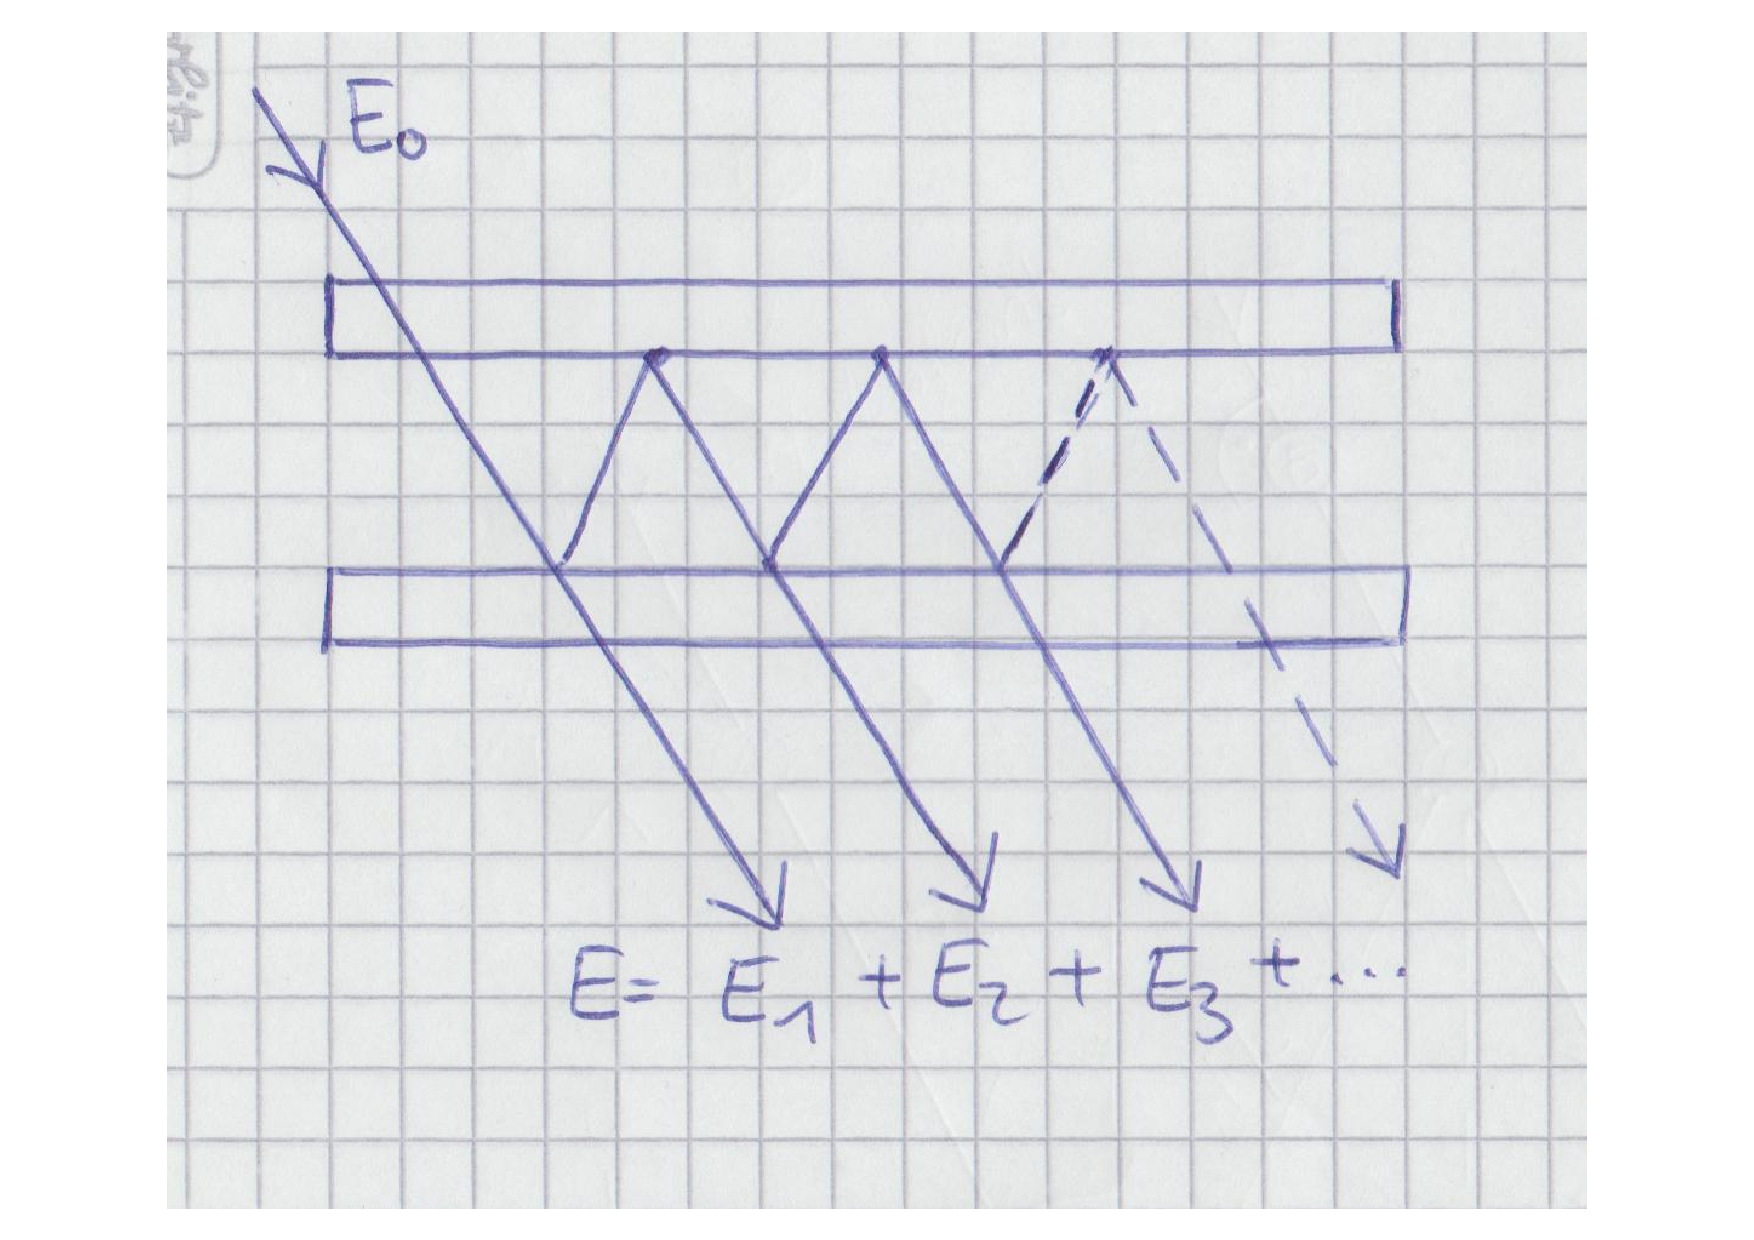
\includegraphics[width=0.9\textwidth]{./Bilder/fp3}
\caption{Vielstrahlinterferenz}
\end{figure}
\FloatBarrier
	
	\section{Fragen zum Versuch}
	\subsection{Aufgabe 1}
	Was sind die wichtigsten Eigenschaften von Laserlicht und wie entsteht Laserlicht? \\
	Laser ist eine Abkürzung für \textbf Light \textbf Amplification by \textbf Stimulated \textbf Emission of \textbf Radiation.\\
	Licht eines Lasers ist Kohärent, insbesondere monochromatisch(zeitliche Kohärenz) und parallel(räumliche Kohärenz).\\
	Laserlicht ist linear polarisiert.\\
	Laserlicht besitzt eine extrem geringe Divergenz.\\
	Die von einem Laser ausgesandten Wellenzüge sind untereinander phasensynchron.\\
	Laserlicht ist sehr gut zu bündeln, daher können hohe Leistungsdichten im Fokus erreicht werden.\\
	Ein Laser besteht aus zwei Spiegeln, den Resonator, von denen ein Spiegel halbdurchlässig ist, einen aktiven Lasermedium, welches je nach Bauart aus einer Gasmischung(CO2 Laser), aus einem Kristallkörper(YAG Laser) oder Glasfasern(Faser Laser) besteht und einer externen Pumpquelle.\\
	Dem Lasermedium wird durch die Pumpquelle Energie zugeführt, wobei das Medium hierdurch angeregt wird und Photonen emittiert. Im Resonator wird die Strahlung des aktiven Lasermediums verstärkt. Gleichzeitig kann nur eine bestimmte Strahlung den Resonator durch den halbdurchlässigen Spiegel verlassen. Diese gebündelte Strahlung ist die Laserstrahlung.\\
	\subsection{Aufgabe 2}
	Muss man den Spiegelabstand vergrössern oder verkleinern, damit sich die Interferenzringe
	zusammenziehen?\\
	Aus der Kreissymmetrie und der Formel für die Transmission
	\[
	T(\alpha)=\frac{T_{max}}{1+F\sin^{2}(2 \pi\frac{d}{\lambda}\cos\alpha)}
	\]
	folgt für zunehmendem Spiegelabstand $d$, ein Zusammenrücken der Ringe.\\
	\subsection{Aufgabe 3} 
	Wie kann man bei bekannter Wellenlänge des verwendeten Lichtes den Verschiebeweg der Spiegel gegeneinander ermitteln? Wie groß ist $\Delta d$, wenn man bei einer Wellenlänge von $\lambda = 500nm$ $200$ periodische Intensitätswechsel beobachtet hat?\\
	Aus der Winkelabhängigkeit der Transmission $T(\alpha)$ sieht man, dass Transmissionsmaxima für solche
	Winkel $\alpha$ entstehen, für die $2d\lambda\cos\alpha$ ganzzahlig ist. Für den $k$-ten Ring (von innen gezählt) gilt
	\[
	\frac{2d}{\lambda}\cos {\alpha}_k=(k_0-k)\qquad k,k_0\in \mathbb{N}
	\]
	Es folgt für $k,l\in \mathbb{N}$ und für feste $d$, $k_0$ und $\lambda$
	\begin{align*}
	(k_0-k)\cos {\alpha}_k &= (k_0-l)\cos {\alpha}_l \\
	\Leftrightarrow\qquad k_0(1-\frac{{ \cos\alpha}_l}{{\cos\alpha}_k}) &= k-l\frac{{\cos\alpha}_l}{{\cos\alpha}_k} \\
	\Leftrightarrow\qquad k_0 &=\frac{k-l\frac{{\cos\alpha}_l}{{\cos\alpha}_k}}{1-\frac{{ \cos\alpha}_l}{{\cos\alpha}_k}}
	\end{align*}
	Es ergibt sich hiermit
	\begin{align*}
	d &=\frac{\lambda}{2}\frac{k_0-k}{\cos {\alpha}_k}\\
	&=\frac{\lambda}{2}\frac{k-l\frac{{\cos\alpha}_l}{{\cos\alpha}_k}-k(1-\frac{{\cos\alpha}_l}{{\cos\alpha}_k})}{(1-\frac{{\cos\alpha}_l}{{\cos\alpha}_k})\cos{\alpha}_k}\\
	&=\frac{\lambda}{2}\frac{{\cos\alpha}_l}{{\cos\alpha}_k}\frac{k-l}{\cos{\alpha}_k-\cos{\alpha}_l}
	\end{align*}
	Aus der Resonanzgleichung \[ n\pi = \frac{2\pi}{{\lambda}_n}d \] folgt
	\begin{align*}
	\Delta d &= \frac{n {\lambda}_1}{2}
	\\ &=\frac{200*500nm}{2}
	\\ &=0,0500mm
	\end{align*}
	n ist dabei die Gesamtzahl der Ringe.
	\\
	\subsection{Aufgabe 4}
	 Wie kann man bei bekannter Spiegelverschiebung $d$ eine unbekannte Lichtwellenlänge bestimmen?\\
	Wie in Aufgabe 3 erläutert mit
	\[
	{\lambda}_1=2\frac{\Delta d}{n}
	\]
	wobei n wieder der Gesamtzahl der Ringe entspricht. \\
	\subsection{Aufgabe 5} 
	Berechnen Sie die Ordnung $k_0$ der zentralen Interferenz ($\alpha=0^\circ$) für $d=3mm$ und $\lambda =600nm$.
	\\Aus der Formel für $T(\alpha=0^\circ)$ folgt, dass für Maxima der Phasenunterschied zwischen zwei benachbarten Teilwellen gleich $\delta=2\pi \frac{2d}{\lambda}$ beträgt, wobei der Spiegelabstand ein ganzzahliges Vielfaches der Wellenlänge sein muss. Hiermit ergibt sich
	\begin{align*}
	k_0 &= \frac{2d}{\lambda}
	\\ &= \frac{2*3mm}{600nm}
	\\ &= 1*10^4
	\end{align*}\\
	\subsection{Aufgabe 6}
	Schätzen Sie den Winkel ab, unter dem dann der erste Inteferenzring ${\alpha}_1$ erscheint.
	\\Für Intensitätsmaximums gilt
	\begin{align*}
	\frac{2d}{\lambda}\cos\alpha=(k_{0}-k)
	\end{align*}
	\\Hiermit ergibt sich
	\begin{align*}
	{\alpha}_1 &=\arccos \frac{\lambda}{2d}
	\\ &=\arccos \frac{600nm}{2*3mm}
	\\ &=1,57
	\end{align*}\\
	\subsection{Aufgabe 7}
	Berechnen Sie das Auflösungsvermögen $\frac{\lambda}{\Delta\lambda}=\frac{\tilde{\nu}}{\Delta\tilde{\nu}}$.\\
	Nach dem Skript gilt (mit F = Finesse)
	\begin{align*}
	F=\frac{\Delta \tilde{\nu}_{FSR}}{\Delta \tilde{\nu}}
	\end{align*}
	\begin{align*}
	\Delta\tilde{\nu}=\frac{\Delta\tilde{\nu}_{FSR}}{F}
	\end{align*}
	Sowie
	\begin{align*}
	F=\frac{\pi\sqrt{R}}{1-R}
	\end{align*}
	und
	\begin{align*}
	\Delta\tilde{\nu}_{FSR}=\frac{1}{2dcos(\alpha)}
	\end{align*}
	Durch einsetzen erhält man nun für das Auflösevermögen:
	\begin{align*}
	\frac{\tilde{\nu}}{\Delta\tilde{\nu}}=\frac{\tilde{\nu}F}{\Delta\tilde{\nu}_{FSR}}=\frac{\pi\tilde{\nu}\sqrt{R}}{(1-R)\Delta\tilde{\nu}_{FSR}}=\frac{2\pi\tilde{\nu}dcos(\alpha)\sqrt{R}}{1-R}
	\end{align*}
	
	\subsection{Aufgabe 8}
	Welchen Nachteil bringt die Erhöhung des Auflösungsvermögens durch Vergrößerung des
	Plattenabstands mit sich?\\
	Aus dem Ergebnis von Aufgabe 7 folgt, dass das Auflösevermögen direkt proportional zum Plattenabstand ist. Durch eine Vergrößerung des Abstands erhöht sich somit auch das Auflösevermögen. Die Vergrößerung des Auflösevermögens auf diesem Weg hat jedoch den Nachteil, dass, wie in Aufgabe 2 gezeigt wurde, bei größerem Abstand das Interferenzmuster dichter wird und somit sehr kleine Ringabstände für die Auswertung gemessen werden müssen.
	
	\subsection{Aufgabe 9}
	Berechnung der Finesse eines Fabry-perot-Interferometers. Wie hängt Finesse mit Anzahl der interferierenden Ringe zusammen?\\
	Laut dem Skript gilt
	\begin{align*}
	F=\frac{\Delta \tilde{\nu}_{FSR}}{\Delta \tilde{\nu}}
	\end{align*}
	somit folgt mit der Erkenntnis aus Aufgabe 7:
	\begin{align*}
	\Delta\tilde{\nu}_{FSR}=\frac{1}{2dcos(\alpha)}
	\end{align*}
	dass
	\begin{align*}
	F=\frac{1}{2dcos(\alpha)\Delta\tilde{\nu}}
	\end{align*}
	Und mit Aufgabe 3 folgt für die Anzahl der Interferenzringe:
	\begin{align*}
	n=(k_{0}-k)=\frac{2d}{\lambda}cos(\alpha)=2d\tilde{\nu}cos(\alpha)
	\end{align*}
	Also ist die Finesse indirekt proportional zur Zahl der Ringe, da diese wiederum direkt proportional zum Ausdruck \(2dcos(\alpha)\) ist. Also steigt die Finesse mit sinkender Ringzahl n.
	\subsection{Aufgabe 10}
	Wie kann man durch Messung der vom Interferometer durchgelassenen minimalen und maximalen
	(abhängig vom Spiegelabstand d) Intensitäten den Reflexionskoeffizienten
	R bestimmen?\\
	\\
	Bei bekannter Ausgangsintensität \(I_{0}\) gilt für die minimale Transmission nach fp.10 im Skript:
	\begin{align*}
	T_{min}=\frac{I_{min}}{I_{0}}
	\end{align*}
	mit fp.13 folgt dann:
	\begin{align*}
	T_{min}=\frac{(1-R)^{2}}{(1+R)^{2}}
	\end{align*}
	\begin{align*}
	T_{min}(1+2R+R^{2})=(1-2R+R^{2})
	\end{align*}
	\begin{align*}
	R^{2}(T_{min}-1)+2R(T_{min}+1)+T_{min}-1=0
	\end{align*}
	Hier bin ich nicht sicher ob das geht:!!!!!!!!!!!!!!!!!!!!!!!!!!!!!!!!!!!!!!!!!!
	Das entspricht mit \(T_{min}=T_{0}=1-R\) und somit \(T_{min}-1=-R\)
	\begin{align*}
	-R^{3}+2R(T_{min}+1)-R=0
	\end{align*}
	\begin{align*}
	-R(R^{2}-1-2T_{min})=0
	\end{align*}
	\begin{align*}
	R^{2}-2T_{min}-1=0
	\end{align*}
	\begin{align*}
	R=\sqrt{2T_{min}+1}
	\end{align*}
	Da aus fp.12 folgt, dass \(T_{max}=1\) muss gelten \(I_{0}=I_{max}\) und somit:
	\begin{align*}
	R=\sqrt{1+2\frac{I_{min}}{I_{max}}}
	\end{align*}
	
\end{document}
